\documentclass{article}
\usepackage[utf8]{inputenc}
\usepackage{amsmath, latexsym}
\everymath{\displaystyle} % better layout

\usepackage{hyperref} % hyperlinks 
\usepackage{xcolor} % colors
\usepackage{graphicx} % figures
\usepackage{caption} % \caption* command in figures

\usepackage[margin=1.3in]{geometry} % smaller margins 



% some math commands
\newcommand{\de}[0]{\mathrm{d}}
\newcommand{\dx}[0]{\de x}
\newcommand{\dt}[0]{\de t}
\newcommand{\ds}[0]{\de s}
\newcommand{\dpartial}[2]{\frac{\partial #1}{\partial #2}}
\newcommand{\dtotal}[2]{\frac{\de #1}{\de #2}}

% a big "to do" signal
\newcommand{\todo}[0]{\colorbox{yellow}{\textcolor{red}{TODO}}}



\setcounter{tocdepth}{4}

\begin{document}

\tableofcontents

\newpage

\section{Foglio 1}
\subsection{1 - Osservatori uniformemente accelerati}
Considero una particella $P_0$, uniformemente accelerata rispetto al sistema istantaneamente inerziale  $\mathcal{I}$.
Il sistema $\mathcal{I}$ va inteso come un insieme di sistemi di riferimento inerziali, tra i quali, per ogni tempo, si considera quello rispetto a cui la particella $P_0$ \`e istantaneamente ferma.
\paragraph{Particella accelerata}
Considero una generica particella $P$, con velocit\`a $u$ e accelerazione $a$ nel sistema $\mathcal{I}$
Scrivo il boost a velocit\`a inversa dal sistema in movimento $\mathcal{I}$ al sistema terra $\mathcal{T}$:
\begin{equation}
	\begin{cases}
		\dx_T = \gamma (\dx + v \dt) &  \\
		\dt_T = \gamma (\dt + v \dt) &  \\ 
	\end{cases}
\end{equation}
\[  u_T = \frac{\dx_T}{\dt_T} = \frac{u+v}{1+uv} \]
\[ \de u_T = \frac{1-v^2}{(1+uv)^2} \de u \]
\begin{equation} \label{accel_P}
	a_T = \frac{\de u_T}{\dt} = \frac{(1-v^2)^{3/2}}{(1+uv)^3} a 
\end{equation}
Volendo trovare la velocit\`a della particella $P_0$, utilizzo l'equazione \ref{accel_P} e la specializzo: la velocit\`a $u$ va posta nulla perch\`e considero la particella $P_0$, ferma in $\mathcal{I}$, e considero l'evoluzione temporale di $v(t_T)$, rispetto al sistema $\mathcal{T}$; la velocit\`a della particella rispetto a $\mathcal{T}$ \`e adesso $v$ e \( a = a_0 \):
\[ a_T = \frac{\de v(t_T)}{\dt_T} = [1-v^2(t_T)]^{3/2} a_0 \]
\[ a_0t_T = \int_0^{v(t_T)} \frac{\de v}{(1-v^2)^{3/2}} \]
sostituisco $v=\sin(\theta)$
\[ a_0t_T= \int_0^{\arcsin(v(t_T))} \frac{\de \theta}{\cos^2(\theta)} = \int \de\tan\theta = \tan(\arcsin(v(t_T))) \]
\[ v(t_T) = \sin(\arctan(a_0t_T)) \]
\begin{equation} \label{veloc}
		v(t_T) = \frac{a_0 t_T}{\sqrt{1+(a_0t_T)^2}} 
\end{equation}

Per trovare la legge oraria, considerando che \(x_T(0)=v_T(0)=0\),
\[ \int_{x_T(0)}^{x_T(t_T)} \dx_T = \int_0^{t_T} \frac{a_0t_T}{\sqrt{a+(a_0t_T)^2}} \dt_T \]
Sostituendo prima \( y=a_0t_T \) e poi \( y = \sinh(z) \) si ottiene
\[ x_T(t_T) = \frac{1}{a_0} \int_{y_0}^y \frac{y}{\sqrt{1+y^2}} \de y \]
\[ = \frac{1}{a_0} \int_{z_0}^z \sinh(z) \de z \]	
\[ = \frac{1}{a_0} [\cosh\sinh^{-1}(y) - \cosh\sinh^{-1}(y_0)] \]
\[ = \frac{1}{a_0} [\cosh(\ln(y + \sqrt{1+y^2}) -1] \]
\[ = \frac{y^2+y\sqrt{1+y^2}+1-y-\sqrt{1+y^2}}{a_0(y+\sqrt{1+y^2})} \]
\[ = \frac{\sqrt{1+y^2}-1}{a_0} \]
\begin{equation} \label{leggeoraria}
	x_T(t_T) = \frac{\sqrt{1+(a_0t_T)^2}-1}{a_0} 
\end{equation}
\todo limite di basse velocit\`a

\paragraph {Achille e la lepre}
Uguagliando c*t a xT dovrei trovare qualcosa, ma se metto c=1 si cancella tquadro e se lo tengo non so dove sbattere la testa.

\paragraph {Tempo proprio}
Con \(\de s^2 = -c^2\dt^2 + \dx^2 \):
\[ ic\de\tau = \de s = ic\dt_T \sqrt(1*-v^2(t_T)) \]
\[ \tau = \int_0^{t_T} \sqrt(1*-v^2(t)) \dt = \int \frac{1}{\sqrt{1+(a_0t)^2}} \dt \]
Sostituendo \( a_0t = \cosh z \)
\[ \tau = \int \frac {\de z}{a_0} = \frac{\sinh^{-1}(a_0t_T)}{a_0} = \frac{\ln({\sqrt{1+(a_0t_T)^2}+a_0t_T)}}{a_0}\]

\paragraph {$10^9$ anni-luce} \todo udm di c
Per percorrere una distanza di $10^9 \mathrm{ly}$ con accelerazione da fermo di \(g=9.8m/s^2=1.030ly/y^2\), usando la formula \ref{leggeoraria}, occorrono
\[ \sqrt{\frac{d}{c}^2 + 2\frac{d}{g}} \simeq 2.998\cdot10^18y \]
cui corrisponde un tempo proprio \( \tau \simeq 41.972 y \).

\paragraph {Perch\`e non andiamo su Giove?}
Con le formule della meccanica classica,
\[ t_{TOT} = 4\cdot \sqrt{\frac{2x_{TM}}{g}} = 2.8558587119250753 y \]
In relativit\`a ristretta, dove 'lh' sono le ore-luce,
\[ t_{TM} = 260.627804384274lh \]
\[ v_{TM} = 0.9999999999999941 c \]
Modificando opportunamente la formula \ref{veloc} per velocit\`a iniziale non nulla, si ottiene
\[ v(t_T) = \frac{a_0 t_T + \tan\arcsin(v_0)          }
	{\sqrt{1+( a_0t_T + \tan\arcsin(v_0)           )^2 }}  \]
\[ v(t_T) = \frac{a_0 t_T + \frac{v_0}{\sqrt{1-v_0^2}} }
	{\sqrt{1+( a_0t_T + \frac{v_0}{\sqrt{1-v_0^2}}  )^2 }}  \]
E per la legge oraria
\[ x_T(t_T) = \frac{\sqrt{1+ (-gt_T + \frac{v_0}{\sqrt{1-v_0^2}})^2 } - 
	\sqrt{1+  (\frac{v_0}{\sqrt{1-v_0^2}})^2}     }{-g} \]
Invertendo:
\[ t = \frac{ \frac{v_0}{\sqrt{1-v_0^2}} + \sqrt{ (\frac{v_0}{\sqrt{1-v_0^2}})^2 - 2gx \sqrt{1+( \frac{v_0}{\sqrt{1-v_0^2}}    )^2     }  } }
             {  g   }\]
\todo risultati bruttissimi

2.99792458e+18  anni
tempo proprio:
41.9715540832882 anni




\paragraph{Razzo relativistico}
Considero il sistema $\mathcal{I}$ in cui il razzo \`e fermo e i sistemi $\mathcal{E}$, in cui \`e ferma la $\de m$ espulsa, e $\mathcal{J}$, in cui \`e fermo il razzo propulso con massa $m-\de m$. Nel sistema $\mathcal{I}$:
\[ \de m v_e \gamma(v_e) = (m - \de m) \de v \gamma(\de v) \sim m \de v \]
\[ \frac{\de m}{m} = \frac{1}{v_e \gamma(v_E)} \frac{\de v}{\de\tau} \de\tau \]
\[ m = m_0 e^{\frac{\frac{\de v}{\de\tau}}{v_e \gamma(v_e) }} \]
\[ m = m_0 e^{\frac{a_0\tau}{v_e \gamma(v_e) }} \]

\paragraph{Campo elettrico}













































\section{Foglio 2}
\subsection{Proiezione stereografica}
Per un cerchio, valgono le relazioni seguenti:
\[ x_{N,S} = R \frac{\sin\theta}{1\mp\cos\theta} \]
Nel caso di una sfera, in coordinate polari tale relazione varra' per il modulo rispetto alla latitudine; la longitudine dara' invece l'argomento. Riscrivendo in campo complesso:
\[ z_{N,S} = \rho_{N,S} e^{i\varphi} \]
\[ \bar{z}_{N,S} = \rho_{N,S} e^{-i\varphi} \]
con 
\[ \begin{cases}
	\rho_{N,S} = R \frac{\sin\theta}{1\mp\cos\theta} & \\
	\varphi_{N,S} = \phi & \\
   \end{cases}
\]


Si definisce la funzione che lega le due carte nel modo seguente:
\[ z_N = \frac{1}{z_S} \]
\[ \bar{z}_N = \frac{1}{\bar{z}_S} \]
Tale relazione \`e olomorfa in \( U_N \cap U_S \), cio\`e il piano complesso senza l'origine e l'infinito.
Le coordinate $w_{N,S}$, ottenute proiettando sul piano tangente alla sfera nel polo opposto, hanno modulo doppio delle rispettive $z_{N,S}$:
\[ w_{N,S} = 2z_{N,S} \]

\subsection{Rotazioni}
I calcoli di questo paragrafo si intendono fatti con $z_N$. % Le derivate si considerano per ora applicate a funzioni olomorfe.
\[ L_z = -i\dpartial{}{\phi} = -i \dpartial{\varphi}{\phi}(\dpartial{z}{\varphi}\dpartial{}{z} + \dpartial{\bar{z}}{\varphi}\dpartial{}{\bar{z}}) = z\dpartial{}{z} - \bar{z}\dpartial{}{\bar{z}}\]
\[ L_\pm = \pm e^{\pm i\phi} (\dpartial{}{\theta} \pm i \cot\theta \dpartial{}{\phi} ) \]
\[ = \pm e^{\pm i\varphi}Re^{i\varphi}  (-\frac{1}{1- \cos\theta} \mp  \cot\theta \frac{\sin\theta}{1-\cos\theta})\dpartial{}{z} \pm e^{\pm i\varphi}Re^{-i\varphi}  (-\frac{1}{1- \cos\theta} \pm  \cot\theta \frac{\sin\theta}{1-\cos\theta})\dpartial{}{\bar{z}} \]

Siccome \( z\bar{z} = \frac{1+c}{1-c}\),
\[ L_+ = -\frac{z^2}{R}\dpartial{}{z} -R\dpartial{}{\bar{z}} , \;\;\;\;\;\;  L_- = R\dpartial{}{z} + \frac{\bar{z}^2}{R}\dpartial{}{\bar{z}} \]
Usando che \( \frac{\partial^2}{\partial z \partial \bar{z}} = \frac{\partial^2}{\partial \bar{z} \partial z}\) 
\[ [L_+,L_-] = 2L_z \]



\subsubsection*{Autovalori di $F_m$}
Tenendo conto che 
\[ L_z f(\rho) = (z\dpartial{\rho}{z} - \bar{z}\dpartial{\rho}{\bar{z}}) \dpartial{f}{\rho} = 0\]
\`e immediato verificare che 
\[ L_z F_m = L_z[z^m] f(\rho) + z^m L_z[f(\rho)] = m F_m\]


\subsubsection*{Forma di $Y_l^l$}
\[ L_+ [f(z\bar{z})] = (-z^2\dpartial{\rho}{z} - \dpartial{\rho}{\bar{z}} ) \dpartial{f}{\rho} \]
\[ = -\frac{z^{m+1}}{R} \left[ mf + (|z|^2+R^2) \dpartial{f}{\rho^2}   \right] \]
Imponendo l'annullamento della parentesi si trova un'equazione differenziale che ha soluzione
\[ f_m (\rho^2) = f_m(\rho^2 + R^2)^{-m} \]
Definendo 
\[ Y_l^m = z^m f_m(\rho^2 + R^2)^{-m}  \]
si vede infine che 
\[ L_+Y^m_l = 0 \iff m=l \]
\[ L_-Y_l^l = (\frac{mR}{z} +\frac{\bar{z}}{R}) Y_l^l \]

Nelle coordinate $(z_S, \bar{z}_S)$
\[ Y_l^m = z_S^{-m}f_m((z_S\bar{z}_S)^{-1} + R^2)^{-m}  \]




\section{Foglio 3}
\subsection{Metrica bidimensionale}
Si studia la metrica
\[ g = \de s^2 = \frac{\epsilon \de x^2 + \de y^2}{y^2} \]
con \( \epsilon = \pm 1\).

\subsubsection*{Vettore di Killing} \todo
Considerando che la metrica non dipende dal modulo di x, ma solo da quello di y, si scrive immediatamente che per 
\[ \vec{k} = \left( \begin{array}{c}  cost \\ 0 \end{array}  \right) \]
\[ \mathcal{L}_{\vec{k}} g = 0 \]

\subsubsection*{Simboli di Christoffel}
L'azione di una particella libera, in parametrizzazione affine, si scrive
\[ S = \frac{1}{2} \int \de \lambda \frac{\epsilon \dot{x}^2 + \dot{y}^2}{y^2} \]
Le variazioni $\delta x$ portano a 
\[ \left(\frac{\epsilon \dot{x}}{y^2}\right)^\cdot = 0 \]
\[ \ddot{x} - \frac{2\dot{x}\dot{y}}{y} = 0 \]
mentre per $\delta y$ si ha
\[ \frac{\epsilon \dot{x}^2 + \dot{y}^2}{y^3} + \left(\frac{\dot{y}}{y^2}\right)^\cdot =0 \]
\[ \ddot{y} + \left(\frac{\epsilon \dot{x}}{y} - \frac{\dot{y}^2}{y} \right) =0 \]
Confrontando le'equazioni con la condizione per le geodetiche
\[ \ddot{x}^\mu + \Gamma^\mu_{\sigma\rho} \dot{x}^\sigma\dot{x}^\rho =0 \]
si trovano
\[ \Gamma^x_{xy} = \Gamma^x_{yx} = -\frac{1}{y} ; \;\;\; \Gamma^y_{xx} = \frac{\epsilon}{y} ; \;\;\; \Gamma^y_{yy} = - \frac{1}{y} \]
Ovvero
\begin{equation}
	\begin{pmatrix}
		\Gamma^x_{\; x} & \Gamma^x_{\; y} \\
		\Gamma^y_{\; x} & \Gamma^y_{\; y} 
	\end{pmatrix} = 
	\begin{pmatrix}
		-\frac{\de y}{y} 	& -\frac{\de x}{y}  \\
		\frac{\epsilon\de x}{y} & -\frac{\de y}{y} 
	\end{pmatrix}
\end{equation}
Con i simboli cos\`i trovati, si possono scrivere le seguenti equazioni
\begin{equation} 
	\begin{cases}
		\nabla e_x = -\frac{\de y}{y} \otimes e_x + \frac{e \de x}{y} \otimes e_y & \\ 
		\nabla e_y = -\frac{\de x}{y} \otimes e_x - \frac{\de y}{y} \otimes e_y & \\
	\end{cases}
\end{equation}

\subsubsection*{Tensore curvatura}
\[ R = \de\Gamma + \Gamma\wedge\Gamma \]
\begin{equation}
	(\de\Gamma)^i_j = \partial_\rho \Gamma_{\mu j}^i \dx^\rho \dx^\mu = \partial_y 
		\begin{pmatrix}
			0 & \frac{1}{y} \\
			-\frac{\epsilon}{y} & 0 \\
		\end{pmatrix}
		\dx\wedge\de y
\end{equation}
\[ (\Gamma\wedge\Gamma)^i_j = \Gamma^i_j\wedge\Gamma^j_k \]
e utilizzando il fatto che 
\[ \dx^\mu\wedge\dx^\mu = 0 = \dx^\mu\wedge\dx^\nu + \dx^\nu\wedge\dx^\mu \]
si trova che \( \Gamma\wedge\Gamma = 0 \).
Ne segue che 
\[ R = \frac{1}{y^2} 
	\begin{pmatrix}
		0 & -1 \\
		\epsilon & 0 \\
	\end{pmatrix}
	\dx\wedge\de y
\]
Il tensore di Ricci \`e 
\[ \mathrm{Ric}_{j\nu} = \delta^\mu_i R^i_{j\mu\nu} \]
E come matrice
\[ \mathrm{Ric} = 
	\begin{pmatrix}
		-\frac{\epsilon}{y^2} & 0 \\
		0                     & -\frac{1}{y^2} \\
	\end{pmatrix}
\]
Lo scalare di curvatura \`e definito come 
\[ R = g^{ij} R_{ij} \]
Si calcola $g^{ij}$ come inverso della metrica, da cui
\[ ||g^{ij}|| = \mathrm{diag}(\frac{y^2}{\epsilon}, y^2) \]
e $R=-2$.

\subsubsection*{Zweibein}
Scrivendo
\[ V^x = \frac{\dx}{y} \;\;\;\;\; V^y = \frac{\de y}{y} \;\;\;\;\; \eta_{ij} = 
	\begin{pmatrix}
		\epsilon & 0 \\
		0        & 1 \\
	\end{pmatrix}
\]
si ha
\[ \de s^2 = \eta_{ij} V^iV^j \]
\newline
Sapendo che 
\[ 	\begin{cases}
	\de V^x = \partial_y \left(\frac{1}{y}\right) \de y \wedge \dx & \\
	\de V^y = \partial_x \left(\frac{1}{y}\right) \dx \wedge \de y = 0  & \\
	\end{cases}
\]
e, considerando \(T^i = 0\), 
\[ \de V^i = -\omega^i_j\wedge V^j \]
(gli indici sono ora intesi nello spazio delle zweibein)
si trova
\[ \omega^y_x \wedge V^x = 0 \]
\[ \omega^x_y \wedge V^y = \frac{1}{y^2} \de y \wedge \dx \]
Considerando che, con la metrica piatta,
\[ V_i = \eta_{ij} V^j = \begin{cases}
	\epsilon V^i & \mathrm{se} \;\; i=x \\
	V^i	     & \mathrm{se} \;\; i=y \\
\end{cases} \]
si trova che 
\[ \omega^x_y \wedge V^y = -V^x\wedge V^y \]
da cui 
\[ \omega^x_y = -V^x \]
e naturalmente
\[ \omega^y_{\,x}= \epsilon\omega^{yx} = -\epsilon\omega^{xy} = -\epsilon\omega^x_{\,y} \]
che verifica la condizione trovata per $\de V^y$.
L'antisimmetria di $\omega^i_{\;j}$ si trasferisce a $R^i_{\;j}$, che avr\`a non nulli solo
\[ R^x_{\;y} = \de \omega^i_{\;j} = -V^x\wedge V^y \;\;\;\;\; R^y_{\;x} = -\epsilon\de \omega^i_{\;j} = \epsilon V^x\wedge V^y \]
Pertanto 
\[ R = \begin{pmatrix}
		0 & -1 \\
		\epsilon & 0 \\
	\end{pmatrix} V^x \wedge V^y \]
Il tensore di Ricci ha componenti
\[ \mathrm{Ric}_{ij} = 
	\begin{pmatrix}
		R^y_{x|yx} & R^x_{x|xy} \\
		R^y_{y|yx} & R^x_{y|xy} \\
	\end{pmatrix}
	= \begin{pmatrix}
		R^x_{\;y} & 0 \\
		0 & R^x_{\;y} \\
	\end{pmatrix}
	= \begin{pmatrix}
		-\epsilon & 0 \\
		0 & -1 \\
	\end{pmatrix}
\]
per cui lo scalare 
\[ R = g^{ij} \mathrm{Ric}_{ij} = -\epsilon^2 -1=-2 \]

\subsubsection*{Derivate covarianti}
I vettori tangenti alle Zweibein sono quelli tali per cui
\[ e_i(V^j) = \delta_i^j \]
e sono pertanto
\[ e_x = y \dx \;\;\;\;\; e_Y = y\de y \]
Se ne calcolano le derivate covarianti, con connessione $\omega^i_{\;j}$:
\[ \nabla e_x = \omega^y_{\;x} e_y = \epsilon e_y \otimes V^x \;\;\;\;\; \nabla e_y = \omega^x_{\;y} e_x =  e_x \otimes V^x \]



\subsubsection*{Integrali primi}
Gli integrali primi
\[ \begin{cases}
	p_x = \frac{\dot{x}}{y^2} & \\
	\sigma = \frac{\epsilon\dot{x}^2 + \dot{y}^2}{y^2} & \\
  \end{cases}
\]
danno le condizioni
\[ \begin{cases}
	\dot{x} = p_x y^2 & \\
	\dot{y}^2 = (\sigma - \epsilon p_x^2 y^2 ) y^2 & \\
  \end{cases}
\]
Si procede calcolando
\[ \left(\frac{\de v}{\dx}\right)^2 = \left( \frac{\de v}{\de \lambda} \frac{\de \lambda}{\dx}  \right)^2 
	= \left( \frac{2\dot{y}y}{\dot{x}} \right)^2 \]
e, sostituendo le condizioni trovate con gli integrali primi, si ottiene
\[ \left(\frac{\de v}{\dx}\right)^2 = \frac{4}{p_x^2} (\sigma - \epsilon\dot{x}^2 y^2 )\]

Per integrare questa equazione,
\[ \frac{\de v}{\dx} = \frac{2}{p_x}\sqrt{\sigma - \epsilon p_x^2 v} \;\;\; \Rightarrow \;\;\;
	\frac{2\sqrt{\sigma}}{p_x} \dx = \frac{\de v}{ \sqrt{1 - \frac{\epsilon p_x^2 v}{\sigma}}} \]
Si sostituisce al secondo membro 
\[ v \rightarrow q = \frac{\epsilon p_x^2 v}{\sigma} \;\;\;\Rightarrow\;\;\; 
	\frac{\sigma}{\epsilon p_x^2} \frac{\de q}{\sqrt{1-q}} \]
Un'ulteriore sostituzione porta a 
\[ q \rightarrow \theta=\arcsin{\sqrt{q}} \;\;\;\Rightarrow\;\;\;
	\frac{2\sigma}{\epsilon p_x^2} \de{\cos\theta} \]
Pertanto, tenendo conto che 
\[ \cos\arcsin\sqrt{q} = \sqrt{1-q} \]
l'integrazione porta a 
\[ \frac{p_x\epsilon}{\sqrt{\sigma}}(x-x_0) = \sqrt{1-\frac{\epsilon p_x^2 v}{\sigma}} -c_0 \]
che raccogliendo le costanti e riarrangiando porta a 
\[ (p_x \epsilon x - K)^2 = \sigma - \epsilon p_x^2v \]
Al variare di $\epsilon$ e $\sigma$, si ottengono i seguenti grafici:
\begin{figure}[htbp]
 \centering
 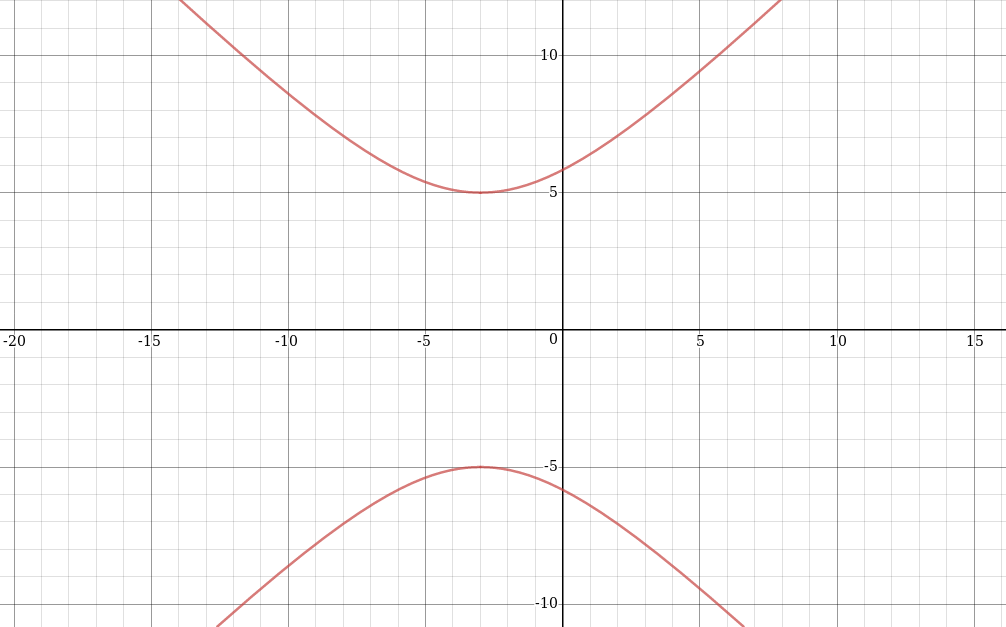
\includegraphics[width=\textwidth]{images/foglio3_neg_neg}
	\caption{\(\epsilon=-1, \;\sigma=-1\)}
 \label{figure:neg_neg}
\end{figure}
\begin{figure}[htbp]
 \centering
 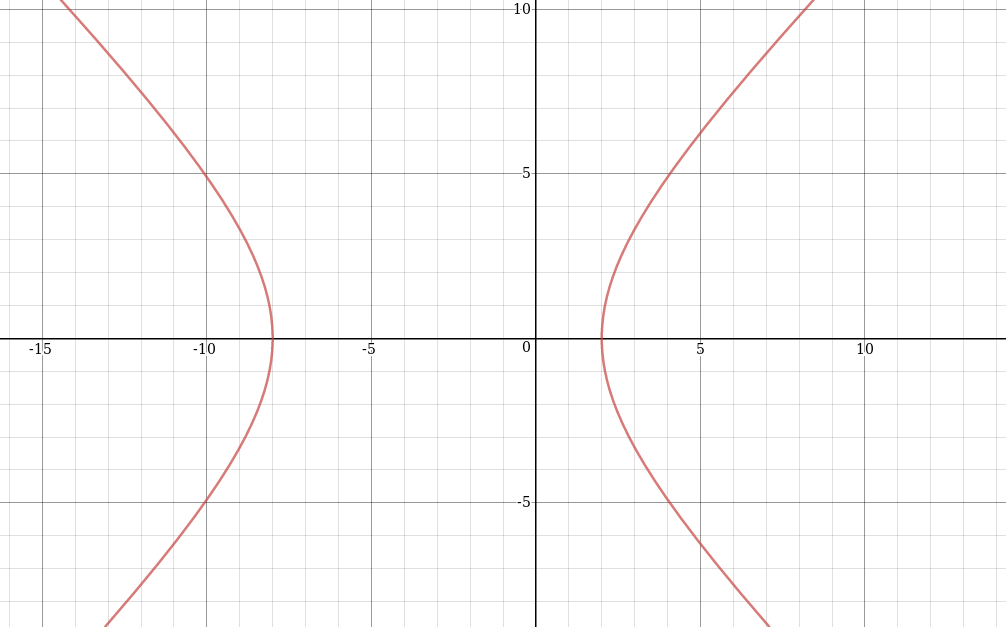
\includegraphics[width=\textwidth]{images/foglio3_pos_neg}
	\caption{\(\epsilon=-1, \;\sigma=+1\)}
 \label{figure:pos_neg}
\end{figure}
\begin{figure}[htbp]
 \centering
 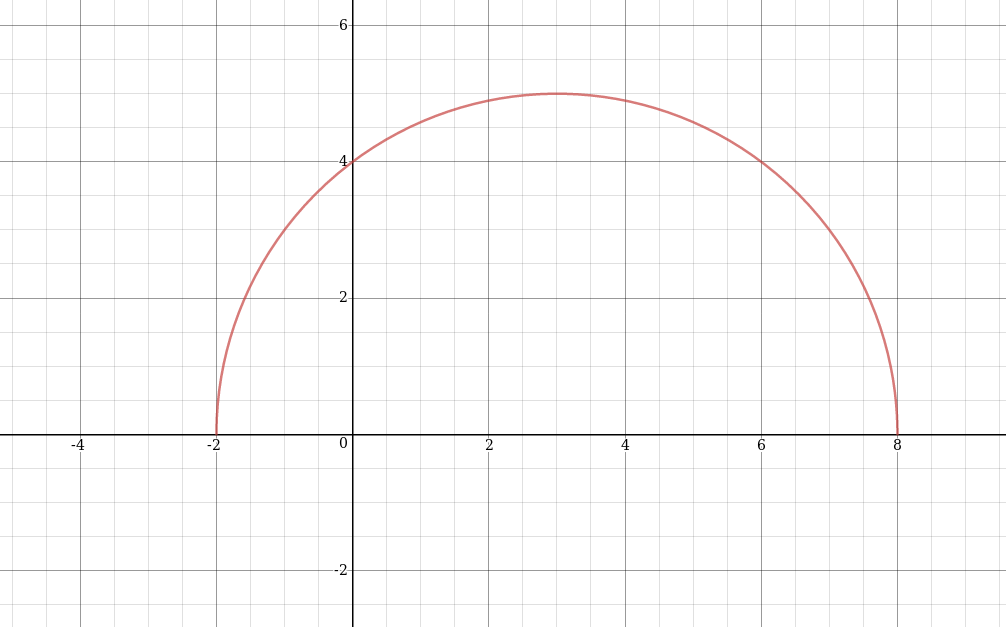
\includegraphics[width=\textwidth]{images/foglio3_pos_pos}
	\caption{\(\epsilon=+1, \;\sigma=+1\)}
 \label{figure:pos_pos}
\end{figure}











\section{Foglio 4}
\subsection{Osservatori in Minkowsky}
Data la metrica 
\[ \de s^2 = -\de t^2 + \dx^2 \]
il cambio di variabili
\[ x = x_0 + vt_0 ; \;\;\; t = t_0 \]
porta, in forma canonica, a 
\[ \de s ^2 = (v^2 -1)\left( \de t_0 + \frac{v}{v^2 -1} \dx_0\right)^2   - \frac{1}{v^2-1} \dx_0^2 \]
da cui si identifica facilmente
\[ \de l^2 = \frac{1}{v^2-1} \dx_0^2 \]
Si pu\`o quindi definire una nuova coppia di variabili, separando la parte spaziale e quella temporale: \( \de X = \de l \).



\subsection{manca}

\subsection{Schwartzschild per osservatori in moto}
Data la metrica di Schwartzschild in D dimensioni
\[  \de s^2 = -c^2 \left( 1- \left(\frac{r_s}{r}\right)^{D-3}\right) \de t^2 + \frac{\de r^2}{1- \left(\frac{r_s}{r}\right)^{D-3}} + r^2 (\de \theta_{D-2} + ...) \]
si calcola il limite di campo debole della sua azione: si considera \( g_{\mu\nu} = \eta_{\mu\nu} + h_{\mu\nu} \) dove $\eta$ \`e la metrica piatta e $h$ rappresenta le perturbazioni gravitazionali, tali che siano infinitesime e dello stesso ordine tra loro.
\[ S = -mc \int \de \lambda \sqrt{- c^2  \left( 1- \left(\frac{r_s}{r}\right)^{D-3} \right)  \dot{t}^2 + g_{ij} \dot{x}^i \dot{x}^j} \]
dove \( \left(\frac{r_s}{r}\right)^{D-3} = \mathcal{O}(|h|) \).
Prendendo \( \lambda = t \) e moltiplicando per 
\( (1-v^2/c^2)^{1/2} (1-v^2/c^2)^{-1/2} \sim \left(1-\frac{v^2}{2c^2}\right) \left(1+\frac{v^2}{2c^2}\right)\)
(dove il quadrato di un vettore indica la sua norma al quadrato) si arriva a 
\[ S = -mc^2 \int \de t  \left(1-\frac{v^2}{2c^2}\right) \left( 1 -\frac{1}{2} \left(\frac{r_s}{r}\right)^{D-3} + \mathcal{O}(\frac{v^2}{2c^2}\cdot |h|) \right) \]
\[ = -mc^2 \int \de t  \left(1-\frac{v^2}{2c^2} -\frac{1}{2} \left(\frac{r_s}{r}\right)^{D-3} \right)\]
\[ = \int \de t \left(  -mc^2  + \frac{1}{2}mv^2 + \frac{1}{2} mc^2\left(\frac{r_s}{r}\right)^{D-3} \right)\]
Identificando i primi due addendi come il termine di massa e quello cinetico, si pu\`o identificare il restante come potenziale gravitazionale, da cui
\[ \frac{1}{2} mc^2\left(\frac{r_s}{r}\right)^{D-3} = -m\phi_{grav} \;\;\Rightarrow \;\;r_s^{D-3} = \frac{2MG_D}{c^2} \]

Si pu\`o definire il cambiamento di coordinate
\[ r^2 = x^2 + \vec{x}^2_\perp \;\;\; ; \;\;\; \cos\theta_{D-2} = \frac{x_{D-1}}{r}  \;\; ; \;\; \cos\theta_{D-3} = \frac{x_{D-1}}{r\cos\theta_{D-2}} \;\; ...\] 
e si vede che 
\[ \sum \de x_i^2 = \de x^2 + \de x^2_\perp = \de r^2 + r^2(\de \theta_{D-2} + \de \theta_{D-3} \sin^2\theta_{D-2} + ... )\]
da cui, raccogliendo $\de r$,
\[  \de s^2 = -c^2 \left( 1- \left(\frac{r_s}{r}\right)^{D-3} \right) \de t^2 
    + \frac{     \left(\frac{r_s}{r}\right)^{D-3} }
           { 1-  \left(\frac{r_s}{r}\right)^{D-3} } \de r^2 
    +  \de x^2 + \de x^2_\perp  \]


\subsubsection{Osservatori in moto}
L'analogo di una trasformazione di Lorentz si ha con
\[ ct = \gamma \frac{1+\beta}{2}U + \gamma \frac{1-\beta}{2}V \;\;\; ; \;\;\; x = \gamma \frac{1+\beta}{2}U - \gamma \frac{1-\beta}{2}V \]
dove U e V sono le coordinate di cono luce. Siccome si vuole determinare la metrica per un osservatore in moto alla velocit\`a della luce,  si pone il limite \( \beta \rightarrow 1 \).
Si scrive la trasformazione dei termini in $\de t$ e $\dx$, per poi imporre le condizioni desiderate:
\[ -c^2 \left( 1- \left(\frac{r_s}{r}\right)^{D-3} \right) \de t^2 +  \de x^2 \] 
\[ \rightarrow \;\;\; \gamma^2 \frac{(1+\beta)^2}{4} \de U^2 + \gamma^2 \frac{(1-\beta)^2}{4} \de V^2 - \de U\de V + \left(\frac{r_s}{r}\right)^{D-3}(\gamma^2 \frac{(1+\beta)^2}{4} \de U^2 + \gamma^2 \frac{(1-\beta)^2}{4} \de V^2 - \de U\de V) \]
Si nota subito che tutti i coefficienti di $\de V$ tendono a zero. Inoltre per \(U\neq 0\)
\[ r = \sqrt{ \gamma^2 (\frac{(1+\beta)^2}{4} U^2 +  \gamma^2 (\frac{(1+\beta)^2}{4} V^2 - UV +   x^2_\perp} \]
che nel limite tende a infinito a causa del $\gamma$ davanti a $U^2$, per cui tutti i termini $\left(\frac{r_s}{r}\right)^{D-3}$ si annullano e rimane
\[ \de s^2 = -\de U\de V + \de x^2_\perp \]
Nel caso in cui \(U=0\), invece, 
\[ r = \sqrt{  x^2_\perp } = x_\perp\]
e 
\[ \de s^2 = \gamma^2  \left(\frac{r_s}{x_\perp}\right)^{D-3} \de U^2 + \mathrm{o}(\de U^2) \]
che diverge nel limite.

\subsubsection{Metrica di Aichelburg-Sexl}
I termini in $\de t$ e $\dx$ si possono riscrivere all'ordine di $\de U^2$, tenendo conto che il termine in $V^2$ svanisce, come
\[ -\de U\de V + r_s^{D-3} \left[ \frac{\gamma^2}{ (\gamma^2 U^2 - UV + x_\perp^2)^{(D-3)/2} } \de U^2 \right] \]
e usando il limite noto \todo RIFERIMENTO 
\[ \left[ \frac{\gamma^2}{ (\gamma^2 U^2 - UV + x_\perp^2)^{(D-3)/2} } \right] =  N_D \frac{\delta{U}}{-UV + x_\perp^{D-4}} =  N_D \frac{\delta{U}}{ x_\perp^{D-4}} \]
inoltre si impone \todo perche'?
\[ \mathrm{lim} M \gamma = M_* \]
per cui 
\[r_s \rightarrow r_{s*} \]
Unendo i risultati \todo e gli altri termini in dr?
\[ \de s^2 = -\de U\de V + N_D r_{s*}^{D-3} N_D \frac{\delta{U}}{ x_\perp^{D-4}} \de U^2 + \de x_\perp^2 \]



\section{Foglio 5}
\subsubsection{Campo debole}
Si considera la metrica D-dimensionale $g_{\mu\nu}$ nell'approssimazione di campo debole.
Le Vielbein possono essere scritte come \( V^a = (\delta^a_\mu + \frac{1}{2} h^a_\mu) \dx^\mu \): si verifica infatti che, al primo ordine in $|h_{\mu\nu}|$, 
\[ \eta_{ab} V^aV^b = g_{\mu\nu}\dx^\mu \dx^\nu \]
Si verifica immediatamente che 
\[ V^\mu_a = (\delta^\mu_a - \frac{1}{2} h^\mu_a) \]
pertanto si pu\`o usare la formula
\[ \omega_{abc} = V^\mu_a V^\nu_b \partial_\mu V^c_\nu - [cab] + [bca] \]
che, considerando di secondo ordine termini del tipo $(\partial h)h$, porta al primo ordine a 
\[ \omega_{abc} = \frac{1}{2} [ \partial{[b} h_{c]a} - [abc] + [cab] \]
\[ \omega_{ab} = \frac{1}{2} \partial_{[b} h_{a]c} V^c \]
Siccome si trascurano termini del tipo $(\partial h)(\partial h)$,
\[ R_{ab} = \de \omega_{ab} = -\frac{1}{2} \partial_i \partial_{[a} h_{b]j} V^i \wedge V^j \]

Lo stesso calcolo si pu\`o fare con i simboli di Christoffel:
\[ \Gamma ^\sigma_{\mu\nu} = \frac{1}{2} g^{\rho\sigma}(\partial_\mu g_{\nu\rho} + [\nu\rho\mu] - [\rho\mu\nu]) = \frac{1}{2}(\partial_\mu h^\sigma_\mu + \partial_\nu h^\sigma_\mu - \partial^\sigma h_{\mu\nu} ) \]
e
\[ R_{\mu\nu} = -\partial_{\alpha} \partial_{[\mu} h_{\nu]\beta} \dx^\alpha \dx^\beta \]

Il tensore di Ricci \`e
\[ Ric_{ab} = - \frac{1}{2} \partial^2  h_{ab} + \frac{1}{2} \partial_\nu \partial^\mu h^b_\mu 
              + \frac{1}{2} \partial_\mu \partial^b h^\mu_\nu - \frac{1}{2} \partial_\nu \partial^b h  \]
che con la gauge 
\[ \partial^a \bar{h}_{ab} = 0  \;\;\; ; \;\;\; \bar{h}_{ab} = h_{ab} - \frac{1}{2} \eta_{ab} h \]
diventa
\[ Ric_{ab} = - \frac{1}{2} \partial^2  h_{ab} \]
da cui il tensore di Einstein \`e immediatamente
\[ G_{\mu\nu} = -\frac{1}{2} \partial^2 \bar{h}_{\mu\nu} \]

\subsubsection{Gauge "di Lorenz"}
Presa una variazione
\[ x'^\mu = x^\mu +\epsilon^\mu(x) \;\;\;\rightarrow \;\;\; \dx'^\mu = \dx^\mu + \partial_\nu \epsilon^\mu \dx^\nu \]
e considerando che la metrica deve restare invariata
\[ g_{\mu\nu}(x)\dx^\mu\dx^\nu = g'_{\mu\nu}(x')\dx'^\mu\dx'^\nu \]
Il primo membro \`e semplicemente \( \eta_{\mu\nu} \dx^\mu\dx^\nu + h_{\mu\nu} \dx^\mu\dx^\nu \), mentre il secondo pu\`o essere espanso al primo ordine come
\[ (g'_{\mu\nu}(x)+\partial_\rho g'_{\mu\nu}(x) \epsilon^\rho)  \dx'^\mu\dx'^\nu = (\eta_{\mu\nu} + h'_{\mu\nu}(x) + \partial_\rho h'_{\mu\nu} \epsilon^\rho) \dx'^\mu\dx'^\nu \]
Quindi uguagliando le due metriche (trascurando i termini $h\epsilon$ o $\partial h\epsilon$)
\[ h_{\mu\nu} \dx^\mu\dx^\nu = \eta_{\mu\nu} \partial_\rho \epsilon^\mu \dx^\rho \dx^\nu + 
                               \eta_{\mu\nu} \partial_\rho \epsilon^\nu \dx^\mu \dx^\rho + 
			       h'_{\mu\nu}(x) \dx^\mu\dx^\nu \]
da cui
\[ h'_{\mu\nu} = h_{\mu\nu} -  \partial_\mu \epsilon_\nu - \partial_\nu \epsilon^\mu \;\;\;;\;\;\;
	\partial^\mu h'_{\mu\nu} = \partial^\mu h_{\mu\nu} - \partial^2 \epsilon_\nu - \partial_\mu \partial_\nu \epsilon^\mu \;\;\;;\;\;\;
	h' = h - 2\partial^\mu \epsilon_\mu \]
e imponendo la gauge
\[ \partial^\mu \bar{h}_{\mu\nu} - \partial^2\epsilon_\nu =0 \]

Per il potenziale Elettromagnetico, invece, 
\[ A'_\mu = A_\mu + \partial_\mu \epsilon \]
e nella gauge di Lorenz
\[ \partial^\mu A_\mu - \partial^2 \epsilon = 0 \]


\subsubsection{Equazioni di Einstein}
In definitiva l'equazione di Einstein diventa
\[ \frac{8\pi G}{c^4} T_{\mu\nu} = G_{\mu\nu} = -\frac{1}{2} \partial^2 \bar{h}_{\mu\nu} \]
\begin{equation} \label{eq:einst_lin}
	\partial^2 \bar{h}_{\mu\nu} = -\frac{16\pi G}{c^4} T_{\mu\nu} 
\end{equation}

\subsubsection{Funzione di Green}
La funzione di Green del D'Alambertiano, valutata nella sua trasformata di Fourier, risulta essere \( \tilde{G} =- 1/k^2 \). Dovendo integrare questa espressione in $k^0$, si nota subito che ha due poli per \( k^0 = |\vec{k}| \), per cui sar\`a necessaria una prescrizione $i\epsilon$, concretizzata in un cambio di variabile \( k^0 -> k^0 \pm i\epsilon \). La richiesta di causalit\`a permette di fissarne il segno, in quanto corrisponde alla richiesta che la funzione sia nulla per \( x^0 < 0\):  infatti, usando il lemma di Jordan, l'integrale in questo intervallo si annulla chiudendo la circonferenza "sopra" l'asse reale; ma, richiedendo che sia nullo, esso non deve contenere i poli, pertanto si ha una situazione come in \ref{figure:green}.


\begin{figure}[htbp]
 \centering
 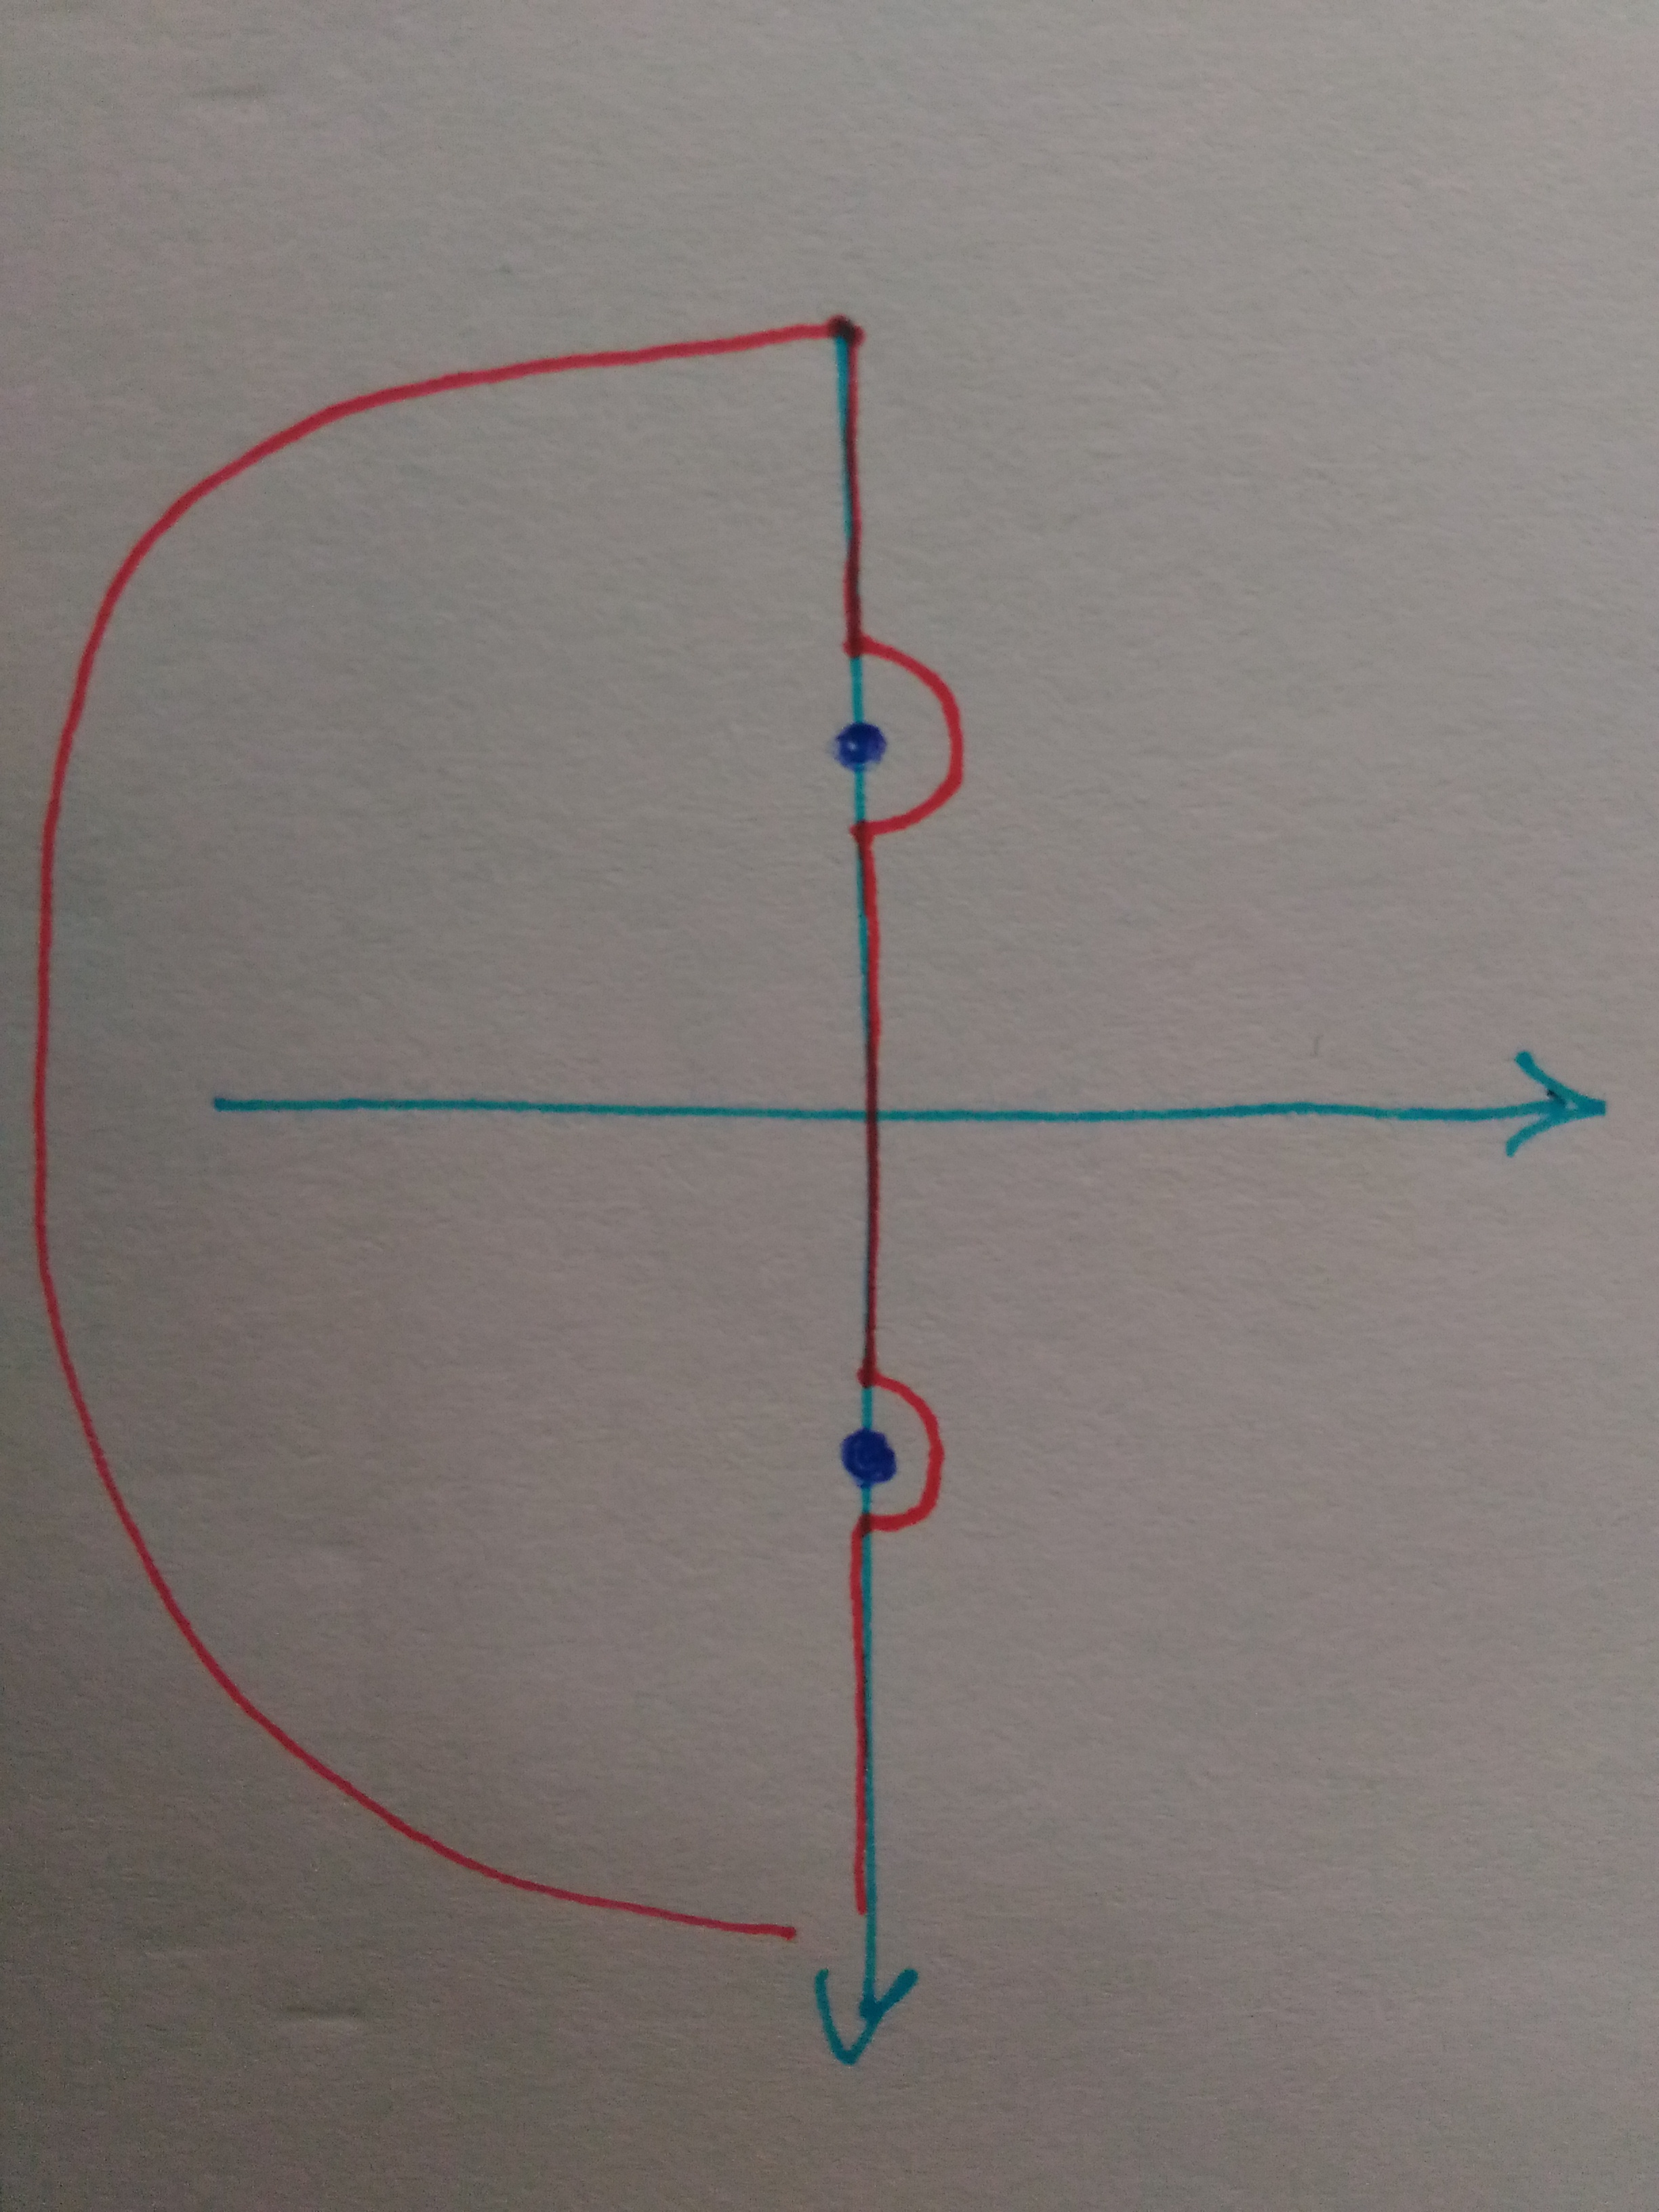
\includegraphics[angle=90, width=0.35\textwidth]{images/foglio5_circuito}
	\caption*{}
 \label{figure:green}
\end{figure}

L'integrale risulta quindi
\[ G_R = \int \frac{\de ^4k}{(2\pi)^4} \frac{e^{ik_\mu x^\mu}}{ (k^0+i\epsilon)^2 - \vec{k}^2 } \]
che diventa col teorema dei residui, in coordinate sferiche
\[ G_R = -\frac{1}{(2\pi)^4} \int \de \phi \; \de \cos\theta \;\de k \;\; k^2 e^{ ik|x|\cos\theta} \frac{2\pi i}{2k} \left[e^{-ikx^0} - e^{ikx^0}\right] \theta(x^0)    \]
\[ G_R = \frac{1}{(2\pi)^2} \frac{1}{2|x|} \int \de k \left( e^{ik|x|} - e^{-ik|x|}\right) \left(e^{-ikx^0} - e^{ikx^0} \right)\theta(x^0)  \]
\[ G_R = \frac{2}{(2\pi)^2 |x|} \int \de k \sin(k|x|) \sin(kx^0) \theta(x^0) \]
Alternativamente, sviluppando i prodotti di esponenziali e cambiando variabile per gli esponenti con segno negativo, utilizzando infine la forma integrale della delta di Dirac \( 2\pi\delta(x) = \int \de k e^{ikx} \) si trova
\[ G_R = -\frac{1}{4\pi|\vec{x}|}\delta{x^0-|\vec{x}|} \]
dove la $\theta$ \`e sottintesa dalla $\delta$.

\subsubsection{Polvere}
Per le propriet\`a della funzione di Green, la \ref{eq:einst_lin} ha soluzione
\[ \bar{h}_{\mu\nu} (x^0,\vec{x}) = \int G_R(x-y) \left[ -\frac{16\pi G}{c^4} T_{\mu\nu}(y) \right] 
		= \frac{4G}{c^4} \int \de ^4y \frac{ T_{\mu\nu}(y) \delta(x^0-y^0-|\vec{x}- \vec{y}|}{|\vec{x}-\vec{y}|} \]
\[ \bar{h}_{\mu\nu} (x^0,\vec{x}) = \frac{4G}{c^4} \int \de ^3y \frac{ T_{\mu\nu}(x^0-|\vec{x}-\vec{y}|, \vec{y})}{|\vec{x}-\vec{y}|} \]

Preso il tensore energia-impulso della polvere
\[ T_{\mu\nu} = (c^2 \rho +p)u_\mu u_\nu + g_{\mu\nu} p \]
nelle condizioni 
\[ u^\mu = (1,\vec{0}) \;\;\; ; \;\;\; |p| << c^2\rho \;\;\; ; \;\;\; \rho = \rho(\vec{y}) \]
Se la materia \`e confinata in un raggio $|\vec{y}_M|$ e il campo viene valutato a distanze molto maggiori di questo raggio, si pu\`o sviluppare
\[ \frac{1}{|\vec{x}-\vec{y}|} \sim \frac{1}{|\vec{x}|} \]
Il tensore energia-impulso si riduce, nelle condizioni date, a
\[ T_{00} = c^2\rho \;\;\; ; \;\;\; T_{ii} = p  \;\;\; ; \;\;\; T = -T_{00} +3 T_{ii} \sim -T_{00} \]
per cui
\[ h_{00} = \bar{h}_{00} + \frac{1}{2} \eta_{00} h = \frac{4G}{c^4|\vec{x}|} \int \de^3y (c^2\rho - \frac{1}{2}c^2\rho) = \frac{2GM}{c^2|\vec{x}|} \]
\[ h_{ii} = \bar{h}_{ii} + \frac{1}{2} \eta_{ii} h = \frac{4G}{c^4|\vec{x}|} \int \de^3y (p + \frac{1}{2}c^2\rho) \sim \frac{2GM}{c^2|\vec{x}|} \]

quindi la metrica diventa
\[ \de s^2 = -(1-\frac{2GM}{c^2r})c^2\de t^2 + (1+\frac{2GM}{c^2r})(\de \vec{x})^2 \]
da cui si vede che, perch\'e resti valido il limite di campo debole, dev'essere
\[ 2GM << c^2r \;\;\;\rightarrow \;\;\; M<<\frac{c^2R}{2G} \]




\subsubsection{Centro di massa nell'origine}
Si prende il centro di massa nell'origine, con velocit\`a nulla. Si considera \( u^\mu \sim (1,\vec{v}/c) \).
\[ T_{00} = c^2\rho \;\;\; ; \;\;\; T_{0i} \sim c\rho v_i \sim T_{00}/c \;\;\; ; \;\;\; T_{ij} \sim \rho v_i v_j\sim T_{00}/c^2 \]
Usando la conservazione di $T_{\mu\nu}$
\[ \partial_\mu T^{\mu\nu} \rightarrow \partial_k T^{k0} = - \partial_0 T^{00} \]
e quindi 
\[ \int_V \de^3y \partial_kT^{0k} y_iy_j = -\int_V \de^3y \partial_0T^{00} y_iy_j  = -\left[ T^{00}y_iy_j\right|_\Sigma + \int \de^3y c^2 T^{00} (v_iy_j + y_iv_j) \]
\begin{equation} \label{eq:commut}
	\partial_0\rho(\vec{y}) = 0 \Rightarrow \partial_0T^{00} = 0 \Rightarrow \int \de^3y T^{00} (v_iy_j + y_iv_j) =0 
\end{equation}
Dove si \`e trascurato il termine di bordo in quanto \todo

Si sviluppa in multipoli
\[ \frac{1}{|\vec{x}-\vec{y}|} \sim \frac{1}{|\vec{x}|} + y^i \frac{x_i}{|\vec{x}|^3} + \mathcal{O}(r^{-5}) \]
da cui
\[ \bar{h}_{00}(x^0,\vec{x}) = \frac{2GM}{c^2 r} + \mathcal{O}(r^{-5}) \]
usando la condizione di massa centrata nell'origine, per cui \( \int \de^3y\rho(\vec{y})y_i = 0\); i termini $T_{ij}$ si trascurano, essendo di ordine $T_{00}/c^2$; infine
\[ \bar{h}_{0i}(x^0,\vec{x}) \sim \frac{4G}{c^3} \int \de^3y 
	\left[ 
		\frac{\rho(\vec{y})v_i}{|\vec{x}|}     
	      - \frac{\rho(\vec{y})v_iy_j x^j}{|\vec{x}|^3} 
	\right] \] 
Il primo termine si annulla: la condizione di centro di massa fermo implica infatti \( \int \de^3y\rho(\vec{y})v_i = 0\). Per quanto riguarda il secondo, grazie a \ref{eq:commut}, si verifica che
\[ \frac{1}{2} \int \de^3y \rho (v_iy_j - y_iv_j) = \int \de^3y \rho v_iy_j \]
pertanto
\[ \bar{h}_{0i}(x^0,\vec{x}) \sim -\frac{2Gx^j}{c^3|\vec{x}|} \int \de^3y \rho(\vec{y}) (v_iy_j - v_jy_i) + \mathcal{O}(r^{-5})  \]
Per cui la metrica diventa, usando \( J_{ij} = \int \de^3y \rho(|\vec{y}|) (v_iy_j - v_jy_i) \),
\[ \de s^2 = -(1 - \frac{2GM}{c^2 r} ) c^2 \de t^2 + (1+\frac{2GM}{c^2 r} ) (\de\vec{x})^2 + \frac{4G}{c^3r^3}J_{ij}\de x^i c \de t + \mathcal{O}(r^-5) \]
\todo perch\`e h00 = hii? 
\todo trascinamento













\end{document}
